\section{Calibration and Selective Prediction}
\textbf{Confidence calibration} is the problem of ensuring the probability estimates predicted by a model accurately reflect the true likelihood of an event occurring. For instance, for 100 predictions provided by a classification model, each with a confidence score of 0.7, we expect that 70 examples should be correctly classified. More formally, we define a perfectly calibrated system as follows:

\begin{gather} \label{eq-cal}
\mathbb{P}(\hat{Y}=Y|\hat{P}=p)=p, \forall p \in [0, 1] 
\end{gather}
where $(\hat{Y}, \hat{P})$ are the predicted labels and confidence scores corresponding to the ground truth $(Y, P)$.

Calibration is essential for many high-stakes applications, such as medical diagnosis, where a poorly calibrated model could lead to incorrect or even dangerous decisions.
However, modern neural networks have been found to be no longer well-calibrated as before, partly due to the increased model capacity and lack of regularization (e.g., normalization, label smoothing, dropout) \citep{guo2017calibration}. 


\paragraph{Measurements of (Mis)Calibration} Expected Calibration Error (ECE) is a commonly used metric to evaluate the miscalibration of a model.
Specifically, ECE first groups predictions into $M$ equally divided interval bins $\{B_{1}, ..., B_{M}\}$, each of size $1/M$. Then, it computes the difference in expectation between the average confidence and the average accuracy. 
Let $B_{m}$ be the bin of samples whose prediction falls into the interval $I_{m} = (\frac{m-1}{M}, \frac{m}{M}]$. ECE is computed as follows:
\begin{gather}
    ECE = \sum_{m=1}^{M} \frac{|B_{m}|}{M}|{\rm acc}(B_{m})-{\rm conf}(B_{m})|, \\
    {\rm acc}(B_{m}) = \frac{1}{|B_{m}|} \sum_{i\in B_{m}}\mathbf{1}(\hat{y}_{i}=y_{i}), \quad
    {\rm conf}(B_{m}) = \sum_{i \in B_{m}} \hat{p}_{i},
\end{gather}
where $\hat{y}_{i}$, $y_{i}$, and $\hat{p}_{i}$ are the predicted label, true label, and confidence for sample $i$. ${\rm acc}(B_{m})$ and ${\rm conf}(B_{m})$ approximate the left-hand and right-hand sides of Eq.(\ref{eq-cal}), respectively. 

In addition, reliability diagrams are a useful visual representation tool for observing calibration. These diagrams plot expected sample accuracy as a function of confidence. In a reliability diagram, ${\rm conf}(B_{m})$ are plotted on the x-axis, and their corresponding ${\rm acc}(B_{m})$ are plotted on the y-axis. Ideally, a well-calibrated model will generate points that fall close to the diagonal line. Any deviation represents miscalibration. An example is presented in \autoref{fig:cal}.

\begin{figure}[ht]
    \centering
    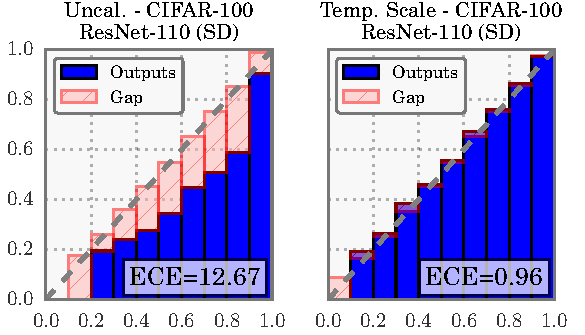
\includegraphics[width=0.6\textwidth]{figures/calibration/reliability_diagram.pdf}
    \caption{Reliability diagram with accuracy on y-axis and model predictive confidence on the x-axis. Temperature scalings leads to lower ECE and better calibration. Taken from \citet{guo2017calibration}.
    }
    \label{fig:cal}
\end{figure}

\paragraph{Calibration Methods}. In addition to regularization that improves calibration during training, various post-processing methods have been proposed to re-calibrate the predicted probabilities. A simple and effective method is temperature scaling which uses a scalar parameter $T>0$ to re-scale the predicted distribution ${\bf p} = softmax({\bf z}/T)$, where ${\bf z}$ is a logit vector. Here $T$ is called the temperature which "softens" the distribution.
Temperature $T$ can also be learned from a set of features $T=f(\phi(x))$, where the feature set $\phi(x)$ typically includes the logits and various task-specific features, e.g., attention weights. 

\paragraph{Structured Calibration} The above definitions and methods are mostly applicable to binary or multi-classification settings. However, in a structured prediction task where the output is a structured label $y=\{y_{1},...,  y_{n}\} \in \mathcal{Y}$, the target space could be prohibitively large. 
\cite{kuleshov2015calibrated} generalized calibration to the structured setting by only considering the calibration of a set of events of interest $\mathcal{I}(x)$. The event set $\mathcal{I}(x)$ can be user-defined, and relevant to the deployment requirements of the system.

\paragraph{Selective prediction} also known as reject option, allows a classifier to abstain from making predictions on low-confidence examples and thereby reduce the error rate. Selective prediction is closely related to confidence calibration, out-of-domain (OOD) detection, and prediction error detection, albeit more remotely.
Formally, a selective classifier comprises a pair of functions $(f, g)$, where $f$ is a standard classifier and $g$ is the selective function: $\mathcal{X} \rightarrow \{0, 1\}$. The output $\hat{y}$ of a selective classifier is computed as follows:
\begin{gather}
\hat{y}=\left\{
\begin{aligned}
f(x) & , & g(x)=1, \\
\varnothing & , & g(x)=0,
\end{aligned}
\right.
\end{gather}
where $\varnothing$ indicates abstention. The selective function $g$ generally consists of a confidence estimator $\tilde{g}: \mathcal{X} \rightarrow \mathbb{R}$ and a threshold $\theta$:
\begin{gather}
    g(x) = \mathbf{1}[\tilde{g}(x) > \theta].
\end{gather}
The confidence estimates $\hat{g}(x)$ can be simply the raw output of the final softmax layer of the classifier or post-processed by calibration methods discussed above.
Intuitively, a selective classifier makes a trade-off between \emph{coverage} and \emph{risk}, which can be computed as:
\begin{gather}
    coverage = \frac{1}{N} \sum_{i=1}^{N} g(x_{i}), \quad risk = \frac{\sum_{i=1}^{N} g(x_{i}) \mathbf{1}[y_{i} \neq \hat{y}_{i}]}{\sum_{i=1}^{N} g(x_{i})},
\end{gather}
where $y_{i}, \hat{y}_{i}$ are the true and predicted labels for example $x_{i}$, respectively.

The performance of a selective classifier can be evaluated by the AUC of the risk-coverage curve (RCC), which is drawn by varying the confidence threshold $\theta$, analogous to ROC curve. 

%\mrinmaya{Could we say something on calibration of language models? We can take some examples from the Neubig paper on QA to contextualize this for LMs? Or Sameer's paper http://proceedings.mlr.press/v139/zhao21c/zhao21c.pdf or maybe something from the Anthopic paper https://arxiv.org/abs/2207.05221 Otherwise this discussion would look like a different train. Doesn't have to be too much more - just 2 paras more with a couple of tables or result figures focused on this would do it.}